\documentclass[12pt]{article}

% Packages
\usepackage[margin=0.6in]{geometry}
\usepackage{graphicx}
\usepackage{amsmath}
\usepackage{float}
\usepackage[dvipsnames]{xcolor}
\usepackage{etoolbox}

\pagestyle{plain}


\begin{document}

\title{Solution ark \#1.\\ Probability sampling. Simple random sampling}
\author{O\u{g}uz--Alper, Melike \& Pekarskaya, Tatsiana, Statistics Norway}
\maketitle

\section*{Exercise 0}

\begin{enumerate}
\item Explain in your own words the reasons why it may be an advantage to select a sample instead of doing a census.\\
\fcolorbox{black}{ForestGreen!20}{
\begin{minipage}[t]{0.97\linewidth} 
\textbf{Solution:}
\begin{itemize}
\item Sampling can provide reliable information at far less cost than a census.
\item Data can be collected more quickly. 
\item Estimates based on sample survey are often more accurate than those based on a census because investigators can be more careful when collecting data. (Lohr, 2019, p.18) 
\item Observations only on a subset of a population provide us a greater scope. Here is meant that you can get more information with a sample rather than with a census, by asking more detailed question in a survey. For a census it is not practical to ask for a detailed information, since it can lead to that one needs ages to publish census' results.  \\
\end{itemize}
\end{minipage}}

\item Discuss the properties of a good sample.\\
\fcolorbox{black}{ForestGreen!20}{
\begin{minipage}[t]{0.97\linewidth} 
\textbf{Solution: }
\begin{itemize}
\item \textit{Goal-oriented}: A sample design should be goal oriented. It is means and should be oriented to the research objectives and fitted to the survey conditions.
\item \textit{Accurate representative of the universe}: A sample should be an accurate representative of the universe from which it is taken. There are different methods for selecting a sample. It will be truly representative only when it represents all types of units or groups in the total population in fair proportions. In brief sample should be selected carefully as improper sampling is a source of error in the survey.
\item \textit{Proportional}: A sample should be proportional. It should be large enough to represent the universe properly. The sample size should be sufficiently large to provide statistical stability or reliability. The sample size should give accuracy required for the purpose of particular study.
\item \textit{Random selection}: A sample should be selected at random. This means that any item in the group has a full and equal chance of being selected and included in the sample. This makes the selected sample truly representative in character. 

\end{itemize}
\end{minipage}}

\fcolorbox{black}{ForestGreen!20}{
\begin{minipage}[t]{0.97\linewidth} 
\begin{itemize}
\item \textit{Economical}: A sample should be economical. The objectives of the survey should be achieved with minimum cost and effort.
\item \textit{Practical}: A sample design should be practical. The sample design should be simple i.e. it should be capable of being understood and followed in the fieldwork.
%\item \textit{Actual information provider}: A sample should be designed so as to provide actual information required for the study and also provide an adequate basis for the measurement of its own reliability.
\end{itemize}
In brief, a good sample should be truly representative in character. It should be selected at random and should be adequately proportional. These, in fact, are the attributes of a good sample. (https://theintactone.com/2019/03/04/brm-u4-topic-3-sample-characteristics-of-a-good-sample/) 
\end{minipage}}
\end{enumerate}

\section*{Exercise 1}

For each survey further, describe the target population, sampling frame, sampling unit and observation unit. Discuss any possible sources of selection bias or inaccuracy of responses:
\begin{enumerate}
\item Potential jurors in some jurisdictions are chosen from a list of county residents who are registered voters or licensed drivers over age 18. In the fourth quarter of 1994, 100 300 jury summons were mailed to Maricopa County, Arizona, residents. Approximately 23 000 of those were returned from the post office as undeliverable. Approximately 7 000 persons were unqualified for service because they were not citizens, were under 18, were convicted felons, or other reason that disqualified them from serving on a jury. An additional 22 000 were excused from jury service because of illness, financial
hardship, military service, or other acceptable reason. The final sample consists of persons who appear for jury duty; some unexcused jurors fail to appear.\\
\fcolorbox{black}{ForestGreen!20}{
\begin{minipage}[t]{0.97\linewidth} 
\textbf{Solution:}\\
\textit{Target population:} Persons eligible for jury duty in Maricopa County.\\
\textit{Sampling frame:} County residents who are registered voters or licensed drivers over
18.\\
\textit{Sampling unit = observation unit:} One resident.\\
\textit{Sources of selection bias or inaccuracy of responses:} Selection bias occurs largely because of undercoverage and nonresponse: 1. Eligible jurors may not appear in the sampling frame because they are not registered to vote and they do not possess an Arizona driver's license. 2.  Addresses on either list may not
be up to date. 3. Jurors fail to appear or are excused (nonresponse). \hfill (Lohr, 2009, p.2)
\end{minipage}}

\item A survey is conducted to find the average weight of cows in a region. A list of all farms is available for the region, and 50 farms are selected at random. Then the weight of each cow at the 50 selected farms recorded.\\
\fcolorbox{black}{ForestGreen!20}{
\begin{minipage}[t]{0.97\linewidth} 
\textbf{Solution:}\\
\textit{Target population:} All cows in region. \\
\textit{Sampling frame:} List of all farms in region. \\
\textit{Sampling unit:} One farm. \\
\textit{Observation unit:} One cow. \\
\textit{Sources of selection bias or inaccuracy of responses:} No selection bias \hfill (Lohr, 2009, pp.2-3) 
\end{minipage}}
\item Kripke et al. (2002) claim that persons who sleep 8 or more hours per night have a higher mortality risk than persons who sleep 6 or 7 hours. They analyzed data from the 1982 Cancer Prevention Study II of the American Cancer Society, a national survey taken by about 1.1 million people. The survival or date of death was determined for about 98\% of the sample six years later. Most of the respondents were friends and relatives of American Cancer Society volunteers; the purpose of the original survey was to explore factors associated with the development of cancer, but the survey also contained a few questions about sleep and insomnia.\\
\fcolorbox{black}{ForestGreen!20}{
\begin{minipage}[t]{0.97\linewidth} 
\textbf{Solution:}\\
\textit{Target population:} All adults \\
\textit{Sampling population:} Friends and relatives of American Cancer Society volunteers \\
\textit{Sampling unit: }One person  \hfill (Lohr, 2009, p.3)
\begin{flushleft}
\small ``\emph{Although the sample contained Americans of diverse ages and backgrounds, and
the sample may have provided valuable information for exploring factors associated
with development of cancer, its validity for investigating the relationship between
amount of sleep and mortality is questionable. The questions about amount of
sleep and insomnia were not the focus of the original study, and the survey was not
designed to obtain accurate responses to those questions. The design did not allow researchers to assess whether the sample was representative of the target population
of all Americans. Because of the shortcomings in the survey design, it is impossible
to know whether the conclusions in Kripke et al. (2002) about sleep and mortality
are valid or not.}"  \\
\footnotesize Lohr, S. (2008). Coverage and sampling, chapter 6 of International Handbook of
Survey Methodology, ed. E. deLeeuw, J. Hox, D. Dillman. New York: Erlbaum, 97-112.
\end{flushleft}
\end{minipage}}
\end{enumerate}

\section*{Exercise 2}
Let $N=6$ and $n=3$. For purposes of studying sampling distributions, assume that all
population values are known. 
\begin{eqnarray*}
y_1=98 \quad y_2=102 \quad y_3=154 \\
y_4=133 \quad y_5=190 \quad y_6=175
\end{eqnarray*}
We are interested in $\bar{y}_U$, the population mean. Two sampling plans are proposed.\\
$\bullet$ Plan 1. Eight possible samples may be chosen.
\begin{center}
\begin{tabular}{ccc}
Sample number & Sample, S & P(S)\\
\hline
1 &\{1,3,5\}& 1/8\\
2 &\{1,3,6\}& 1/8\\
3 &\{1,4,5\}& 1/8\\
4 &\{1,4,6\}& 1/8\\
5 &\{2,3,5\}& 1/8\\
6 &\{2,3,6\}& 1/8\\
7 &\{2,4,5\}& 1/8\\
8 &\{2,4,6\}& 1/8\\
\end{tabular}
\end{center}
$\bullet$ Plan 2. Three possible samples may be chosen.

\begin{center}
\begin{tabular}{ccc}
Sample number & Sample, S & P(S)\\
\hline
1 &\{1,4,6\}& 1/4\\
2 &\{2,3,6\}& 1/2\\
3 &\{1,3,5\}& 1/4\\
\end{tabular}
\end{center}

\begin{enumerate}
\item What is the value of $\bar{y}_U$?\\
\fcolorbox{black}{ForestGreen!20}{
\begin{minipage}[t]{0.97\linewidth} 
\textbf{Solution:} $\bar{y}_U=\sum_{i=1}^Ny_i/N=142$  
\end{minipage}}
\item Let $\bar{y}$ be the mean of the sample values. For each sampling plan, find \\
(i) $E(\bar{y})$; (ii) $V(\bar{y})$; (iii) Bias($\bar{y}$); (iv) MSE($\bar{y}$).\\

\fcolorbox{black}{ForestGreen!20}{
\begin{minipage}[t]{0.97\linewidth}
\textbf{Solution:}\\
\textit{Plan 1}\\
First, let's calculate $\bar{y}_S$ for each sample $S$:
$\bar{y}_{S1} = 1/3(y_1 + y_3 + y_5) = 1/3(98 + 154 + 190) = 147.33$
Results for other sample you can find in the table:  
\begin{center}
\begin{tabular}{cccc}
Sample number & Sample, S & P(S) & $\bar{y}_S$ \\
\hline
1 &\{1,3,5\}& 1/8&147.33\\
2 &\{1,3,6\}& 1/8&142.33\\
3 &\{1,4,5\}& 1/8&140.33\\
4 &\{1,4,6\}& 1/8&135.33\\
5 &\{2,3,5\}& 1/8&148.67\\
6 &\{2,3,6\}& 1/8&143.67\\
7 &\{2,4,5\}& 1/8&141.67\\
8 &\{2,4,6\}& 1/8&136.67\\
\end{tabular}
\end{center}
Further we get:\\
(i) $E(\bar{y}) = \sum_{S}\bar{y}_S P(S)=\frac{1}{8}147.33+\frac{1}{8}142.33+\cdots+\frac{1}{8}136.67=142$ \\
(ii) $V(\bar{y}) = \sum_{S}[\bar{y}_S-E(\bar{y})]^2 P(S)=\frac{1}{8}(147.33-142)^2+\frac{1}{8}(142.33-142)^2+\cdots+\frac{1}{8}(136.67-142)^2=18.94$ \\
(iii) $\mathrm{Bias}(\bar{y})=E(\bar{y})-\bar{y}_U=142-142=0$ \\
(iv) $\mathrm{MSE}(\bar{y})=\mathrm{Bias}(\bar{y})^2+V(\bar{y})=18.94$. \\

\textit{Plan 2}\\
\begin{center}
\begin{tabular}{cccc}
Sample number & Sample, S & P(S) & $\bar{y}_S$\\
\hline
1 &\{1,4,6\}& 1/4&135.33\\
2 &\{2,3,6\}& 1/2&143.67\\
3 &\{1,3,5\}& 1/4&147.33\\
\end{tabular}
\end{center}
(i) $E(\bar{y})=\frac{1}{4}135.33+\frac{1}{2}143.67+\frac{1}{4}147.33=142.5$ \\
(ii) $V(\bar{y})=\frac{1}{4}(135.33-142.5)^2+\frac{1}{2}(143.67-142.5)^2+\frac{1}{4}(147.33-142.5)^2=19.36$ \\
(iii) $\mathrm{Bias}(\bar{y})=142.5-142=0.5$ \\
(iv) $\mathrm{MSE}(\bar{y})=0.5^2+19.36=19.6$. \\
\end{minipage}}
\item Which sampling plan do you think is better? Why?\\
\fcolorbox{black}{ForestGreen!20}{
\begin{minipage}[t]{0.97\linewidth}
\textbf{Solution:} Sampling Plan 1 is better as it has smaller variance and provides unbiased estimation.
\end{minipage}}
\end{enumerate}

\section*{Exercise 3}
\textbf{\color{ForestGreen}(R code available for parts 3 - 5)} Let  $U$ be a population of size $N=8$ with the index set $U = \{1, 2, 3, 4, 5, 6, 7, 8\}$. The values of $y_i$ are 
\begin{center}
\begin{tabular}{ccccccccccc}
$i$ & \vline & 1 & 2 & 3 & 4 & 5 & 6 & 7 & 8 \\
\hline
$y_i$ & \vline &  1 & 2 & 4 & 4 & 7 & 7 & 7 & 8
\end{tabular}
\end{center}

For this population, consider sampling scheme 
\begin{center}
\begin{tabular}{cc}
$S$ & $P(S)$\\
\hline
\{1,3,5,6\}& 1/8\\
\{2,3,7,8\}& 1/4\\
\{1,4,6,8\} &1/8\\
\{2,4,6,8\} &3/8\\
\{4,5,7,8\} &1/8\\
\end{tabular}
\end{center}
\begin{enumerate}
\item Find the probability of selection $\pi_i$ for each unit i.\\
\fcolorbox{black}{ForestGreen!20}{
\begin{minipage}[t]{0.97\linewidth}
\textbf{Solution:}\\
$\pi_i = \sum_{S_q}\ I_i P(S_q)$, where $\ I_i = 1$ if $i$ in $S_q$, and $\ I_i=0$ otherwise  \\
For $i=1$ we have, \\
$\pi_1 = P(S_1) + P(S_3) = 1/8 + 1/8 = 0.25$ \\ 
The rest can be found similarly. You should get 
$\pi_2 = \pi_4 = \pi_6 = 0.625$, $\pi_3 = \pi_7 = 0.375$, $\pi_5 = 0.25$ and $\pi_8 = 0.875$
\end{minipage}}
\item What is the sampling distribution of $\hat{t} = 8\bar{y}$? \\
\fcolorbox{black}{ForestGreen!20}{
\begin{minipage}[t]{0.97\linewidth}
\textbf{Solution:}\\
$8\bar{y}_{S_1} = 8(1 + 4 + 7 + 7)/4 = 38$,\\
and the rest can be found similarly\\ 
$8\bar{y}_{S_2} = 8\bar{y}_{S_4} = 42$,\\ $8\bar{y}_{S_3} = 40, 8\bar{y}_{S_5} = 52$.\\
The sampling distribution of $8\bar{y}$ is \\

\begin{center}
\begin{tabular}{cccccc}
$k$ & \vline & 38 & 40 & 42 & 52\\
\hline
$P(8\bar{y}=k)$ & \vline & 1/8 & 1/8 & 5/8& 1/8 \\ 
\end{tabular}
\end{center}
To understand how sampling distribution of mean is obtained one can try to play in a tool (http:// onlinestatbook.com/stat\_sim/sampling\_dist/index.html). The tool can help to understand several concepts regarding sampling by visualising them. \\
\end{minipage}}
\item Assume a SRS of size 3 without replacement and find expectation and variance of $\bar{y}$\\
\fcolorbox{black}{ForestGreen!20}{
\begin{minipage}[t]{0.97\linewidth}
\textbf{Solution:}\\
Number of all possible samples of size $n=3$ selected from $U$ of size $N=8$ under SRSWOR is \\
$\binom{8}{3}=\frac{8!}{3!(8-3)!}=56$ \\ 
$E_{srswor}(\bar{y})=\bar{Y} = 5$ \\
Analytical variance calculation: \\
$V_{srswor}(\bar{y})=(1-\frac{n}{N})\frac{1}{n}S^2=1.429$,  \\
where $S^2=\frac{1}{N-1}\sum_{i\in U}(y_i-\bar{Y})^2 = 6.857143$
\end{minipage}}

\item Assume a SRS of size 3 with replacement and find expectation and variance of $\bar{y}$.\\
\fcolorbox{black}{ForestGreen!20}{
\begin{minipage}[t]{0.97\linewidth}
Number of all possible samples of size $n=3$ selected from $U$ of size $N=8$ under SRSWR is \\
$8^3=512$ \\
$E_{srswr}(\bar{y}) = E_{srswor}(\bar{y})=\bar{Y} = 5$\\
Analytical variance calculation: \\
$V_{srswr}(\bar{y})=\frac{1}{n}\frac{\sum_{i\in U}(y_i-\bar{Y})^2}{N}=\frac{N-1}{N}\frac{1}{n}S^2=2$,\\
where $S^2=6.857143$
\end{minipage}}

\item For 3. and 4., draw the histogram of the sampling distribution of $\bar{y}$. Which sampling distribution has the smaller variance, and why?\\
\fcolorbox{black}{ForestGreen!20}{
\begin{minipage}[t]{0.97\linewidth}

\begin{figure}[H]
\begin{center}
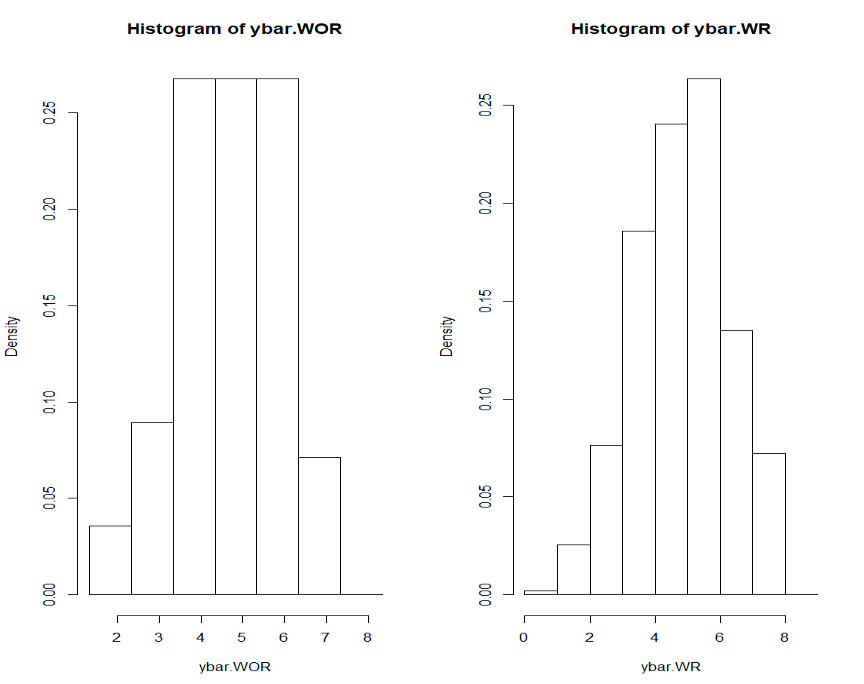
\includegraphics[scale=0.6]{Ex3_5.png}
\end{center}
\end{figure}

Variance of SRSWOR is smaller than variance of SRSWR:\\
$V_{srswor}=(1-\frac{n}{N})\frac{1}{n}S^2$\\
$V_{srswr}=(1-\frac{1}{N})\frac{1}{n}S^2$\\
$\frac{n}{N} > \frac{1}{N}$ for $n > 1$\\
$ 1 - \frac{n}{N} < 1 - \frac{1}{N}$

\end{minipage}}

\end{enumerate}


\section*{Exercise 4}
\textbf{\color{ForestGreen}(R code available)} A university has 807 faculty members. For each faculty member, the number of refereed publications was recorded. This number is not directly available on the database,
so requires the investigator to examine each record separately. A frequency table for number of refereed publications is given below for an SRS of 50 faculty members.

\begin{center}
\begin{tabular}{lrrrrrrrrrrrr}
Refereed Publications & \vline & 0& 1& 2& 3& 4& 5& 6& 7& 8& 9& 10 \\
\hline
Faculty Members & \vline &  28& 4& 3& 4& 4& 2& 1& 0& 2& 1& 1\\
\end{tabular}
\end{center}

\begin{enumerate}
\item Plot the data using a histogram. Describe the shape of the data.\\
\fcolorbox{black}{ForestGreen!20}{
\begin{minipage}[t]{0.97\linewidth}
\textbf{Solution:} 
\begin{figure}[H]
\begin{center}
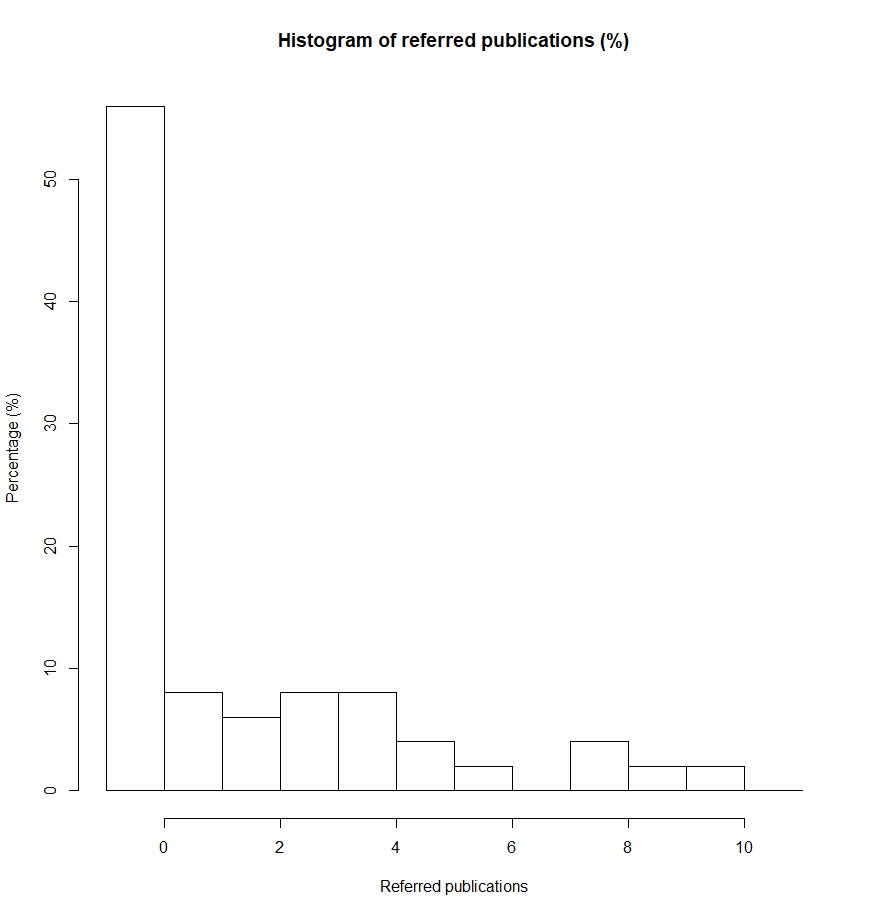
\includegraphics[width=0.6\textwidth]{Ex4_1}
\end{center}
\end{figure}
\end{minipage}}

\item Estimate the mean number of publications per faculty member, and give the SE for your estimate.\\
\fcolorbox{black}{ForestGreen!20}{
\begin{minipage}[t]{0.97\linewidth} 
\textbf{Solution:}\\
From problem statement we know that $N = 807$ and $n = 50$ \\
$\bar{y} =(28*0+4*1+\dots+1*10)/50=1.78$ \\
$\mathrm{\widehat{SE}(\bar{y})} = \sqrt{((1-f)s^2/n)}$ where $s^2 = 1/(n-1) \sum_{i \in s}[y_i-\bar{y}]^2$. \\
Applying the formulas we get \\
$\quad s^2=1/49*[28*(0-1.78)^2 + 4(1 - 1.78)^2 + \dots + 1*(10-1.78)^2] = 7.1955$ and \\
$\mathrm{\widehat{SE}(\bar{y})} =\sqrt{((1-50/807)s^2/50)}=0.367$ \\
\end{minipage} 
}


\item Do you think that $\bar{y}$ from 2. will be approximately normally distributed? Why or why not?\\
\fcolorbox{black}{ForestGreen!20}{
\begin{minipage}[t]{0.97\linewidth} 
\textbf{Solution:} 
Probably not as the original data is quite skewed and a sample size of $n=50$ may not be large enough to get a normal distribution for $\bar{y}$ over repeated sampling. We can use the formula (2.23) (Lohr, 2019. p.44) to calculate an adequate sample size to get a normal distribution:
$$n_{min}=28+25\,\hat{\gamma}^2, \quad \hat{\gamma}=\hat{\mu}_3/\hat{\mu}_2^{3/2},$$
where $\hat{\gamma}$ is an estimate of an measure of skewness, and $\hat{\mu}_2$ and $\hat{\mu}_3$ are the estimates of the second and the third central moments defined by:
$$\hat{\mu}_2=s^2$$ and $$\hat{\mu}_3=1/n\sum_{i \in s}(y_i-\bar{y})^3$$ \\
We have $\hat{\mu}_2=s^2=7.1955$ and $\hat{\mu}_3=28.9247$, and so 
$\hat\gamma=28.9247/7.1955^{3/2}=1.5$ (to calculate this there is available function "\emph{skewness}" in R package "\textbf{e1071}")\\
Then we get that an adequate sample size is:\\
$n_{min}=\lceil28+25*1.5^2\rceil=85$ which is larger than a give sample size $n = 50$.
\end{minipage}}

\item Estimate the proportion of faculty members with no publications and give a 95\% confidence interval. \\
\fcolorbox{black}{ForestGreen!20}{
\begin{minipage}[t]{0.97\linewidth}
\textbf{Solution:} 
Proportion of faculty members is:\\
$\hat{p}_{nopub}=28/50=0.56$ \\
To calculate CI, first, we need to calculate SE:\\
$$\widehat{SE}(\hat{p}_{nopub})=\sqrt{(1-f)\frac{\hat{p}_{nopub}(1-\hat{p}_{nopub})}{(n-1)}}$$
$\widehat{SE}(\hat{p}_{nopub})=\sqrt{(1-50/807)0.56(1-0.56)/49}=0.0687$\\
Then $95\%\,\mathrm{CI}: [0.56\mp 1.96*0.0687]=[0.425;0.695]$
\end{minipage}}
\end{enumerate}


\section*{Exercise 5}
A typical opinion poll surveys about 1000 adults. Suppose that the sampling frame contains 100 million adults including yourself, and that an SRS of 1000 adults is chosen from the frame.
\begin{enumerate}
\item What is the probability that you are selected to be in the sample?\\
\fcolorbox{black}{ForestGreen!20}{
\begin{minipage}[t]{0.97\linewidth}
\textbf{Solution:} \\
From problem statement we have $n=1000$, $N=100\,000\, 000$ and SRS\\
We can simply use the formula of probability $\pi$ under SRS, that is,\\ $\pi=n/N=1000/100\,000\,000=1/100\,000$.\\
Alternatively we could use the theory of probability:
$$P(I_i=1)=\frac{\binom{N-1}{n-1}}{\binom{N}{n}} = \frac{(N-1)!}{(n-1)!(N-n)!}\Big(\frac{N!}{n!(N-n)!}\Big)^{-1}=\frac{n}{N}$$
\end{minipage}}
\item Now suppose that 2000 such samples are selected, each sample selected independently of the others. What is the probability that you will not be in any of the
samples?\\
\fcolorbox{black}{ForestGreen!20}{
\begin{minipage}[t]{0.97\linewidth}
\textbf{Solution:} \\
 $P[(1-\mathrm{I}_{i;S_1})(1-\mathrm{I}_{i;S_2})\cdots (1-\mathrm{I}_{i;S_{2\,000}})=1]=(1-\pi)^{2\,000}=0.9801986$,
 \\ where $\mathrm{I}_{i;S_q}=1$ if $i \in S_q$, and $\mathrm{I}_{i;S_q}=0$ otherwise, with $q=1,2,\cdots,2\,000$. 
\end{minipage} }
\item How many samples must be selected for you to have a 0.5 probability of being in at least one sample?\\
\fcolorbox{black}{ForestGreen!20}{
\begin{minipage}[t]{0.97\linewidth}
\textbf{Solution:} \\
{\small P($i$ in at least one sample among $q$ samples) = 1-P($i$ not in any of the $q$ samples)}\\
P($i$ not in any of the $q$ samples) = 0.5
$$P[\pi_{S_q}(1-\mathrm{I}_{i;S_{q}})=1]=(1-\pi)^q=0.5$$ 
Taking logarithm of both sides, we obtain \\
$q\log{(1-1/100\,000)}=\log{0.5}$\\
$q=\log{0.5}/\log{0.99999}=69\,314.37$
\end{minipage} }
\end{enumerate}

\section*{Exercise 6}
It is important to keep track on unemployment level from month to month. Let’s assume that you have been assigned a task to find a size of SRS n. You have no idea about the proportion of unemployed people in the population, but you read in literature that p = 0.5 is often used when you have no idea about the value of proportion. So you decide to use as p = 0.5. Assume that population size is large and, thus, you can ignore fpc. You work with 95\% confidence level.
\begin{itemize}
\item What is the value of n if your margins of error is c 0.001, 0.002, 0.005? \\
\fcolorbox{black}{ForestGreen!20}{
\begin{minipage}[t]{0.97\linewidth}
\textbf{Solution:} \\
From $1.96 * \sqrt{\frac{(1-p)p}{n}} = c$, we get that $n = 1.96^2(1-p)p/c^2$.\\
Then n for different c values are:
\begin{center}
\begin{tabular}{cc}
$c$ & $n$\\
\hline
0.001 & 960\,400\\
0.002 & 240\,100\\
0.005 & 38\,416\\
\end{tabular}
\end{center}
\end{minipage} }


\item	Why proportion of interest p = 0.5 is often used when one does not have an idea about the value of the proportion?\\
\fcolorbox{black}{ForestGreen!20}{
\begin{minipage}[t]{0.97\linewidth}
\textbf{Solution:} \\
0.5 is often used when you have no idea about the value of the proportion of interest as 0.5 would provide a conservative result (highest variance leading to largest sample size for a given margin of error).
To find it we fix c value in $n = 1.96^2(1-p)p/c^2$ and take a derivative: $((1-p)p)'=(p-p^2)'=1-2p$. An extreme value will be where $1-2p=0 \implies p = 1/2$.
\end{minipage} }
\end{itemize}

\end{document}